\section{El Potato}

Con la muerte del "Potato" se llevará a cabo un nuevo cónclave en el Vaticano, en el que participan todos los cardenales  del mundo. Sin embargo, también se sabe que, esta vez, existe un participante nuevo que afirma ser un dios en la tierra y merecer ser el nuevo "Potato"; estamos hablando de Sentry, el cual decide meterse a la fuerza al Vaticano y participar de la votación. Sentry ha mandado a algunos Thunderbolts a averiguar como es la vuelta allá en Roma. Ghost se metió de infiltrada a los archivos del Vaticano y descubrió que los votos por los cuatro principales candidatos se encuentran al resolver el siguiente sistemas de ecuaciones.

\[
\underbrace{\begin{bmatrix}
118 &  1 & 10 &  2\\
  8 & 119 &  1 & 10\\
10 &  9 & 100 & 3\\
  5 &  9 & 10 & 113
\end{bmatrix}}_{A}
\;
\underbrace{\begin{bmatrix}
x_1\\ x_2\\ x_3\\ x_4
\end{bmatrix}}_{\mathbf{x}}
\;=\;
\underbrace{\begin{bmatrix}
1000\\ 2000\\ 3000\\ 4000
\end{bmatrix}}_{\mathbf{b}}
\]


Donde $x_i$ corresponde a los votos recibidos por cada candidato y $cc$
corresponde al número 10.

Ayude a Sentry a saber si tiene futuro como "Potato".

%======================================================================
\section{1. (1.5 pt) Encontrar los votos recibidos}

Encuentre los votos recibidos por los cuatro principales candidatos usando el
método de SOR con: condición inicial \(X_0=\mathbf b\), tolerancia de
tres cifras significativas \((\text{tol}=10^{-3})\) y parámetro
\(\omega = 1.15\).  El error a controlar debe ser

\[
\Bigl\|\,\bigl(X^{(k)}-X^{(k-1)}\bigr)\!./X^{(k)}\Bigr\|_2 .
\]

%----------------------------------------------------------------------
\subsection*{Código ejecutado en \texttt{Matlab Online}}

\begin{lstlisting}[language=Matlab,basicstyle=\ttfamily\small]
% Matriz y termino independiente
A = [118  1  10   2;
      8 119   1  10;
     10   9 100   3;
      5   9  10 113];
b = [1000; 2000; 3000; 4000];

% Parametros SOR
x0    = b;      % X0 = b
Tol   = 1e-3;   % 3 cifras significativas
niter = 100;    % maximo de iteraciones
w     = 1.15;   % factor de relajacion

% Ejecucion
[E,x] = SOR(x0,A,b,Tol,niter,w);   % rutina con norma 2
votes = round(x);                  % votos enteros
T     = table((1:numel(E))',E',...
              'VariableNames',{'k','Error'});
disp(votes), disp(T)
\end{lstlisting}

\vspace*{-1ex}
%----------------------------------------------------------------------
\paragraph{Convergencia.}
El algoritmo terminó en \(9\) iteraciones (se alcanza
\(\|\,\cdot\,\|_2<10^{-3}\) en la novena).  
La evolución del error fue:

\[
\begin{array}{|c|c|}
\hline
k & \bigl\|(X^{(k)}-X^{(k-1)}) ./ X^{(k)}\bigr\|_2\\\hline
1 & 1.3797\times10^{1}\\
2 & 1.2397\times10^{1}\\
3 & 1.4734\times10^{1}\\
4 & 4.1671\\
5 & 1.7001\\
6 & 2.0311\times10^{-1}\\
7 & 2.6545\times10^{-2}\\
8 & 2.7298\times10^{-3}\\
9 & 1.7292\times10^{-4}\\\hline
\end{array}
\]

%----------------------------------------------------------------------
\paragraph{Votos obtenidos.}
La solución aproximada al sistema lineal es
\[
\mathbf{x}\approx
\begin{bmatrix}
 3.6485\\ 10.2824\\ 20.8509\\ 24.4684
\end{bmatrix},
\qquad
\text{lo que redondea a}\;
\boxed{[\,4,\;10,\;21,\;24\,]^{\mathsf T}}.
\]

\begin{itemize}
  \item \textbf{Sentry} (\(x_1\)) obtiene \textbf{4 votos}.
        No hay conteos negativos, de modo que (por ahora) no necesita
        ``dar de baja'' a ningún cardenal.
  \item El error pedido desciende por debajo de \(10^{-3}\) en la iteración 9,
        lo que confirma la convergencia con el umbral exigido.
\end{itemize}

\noindent
Con únicamente cuatro votos sobre más de cuatro mil, el autoproclamado
dios-en-la-tierra sigue muy lejos de convertirse en el nuevo \emph{Potato}.

\section{2. (1.5 pt) Interpolar los datos y calcular la cantidad de votos obtenidos}

Al final resulta que había un quinto candidato con altas posibilidades de ganar,
un tal "Roberto Prevoto", que debido a su nombre ya tenía conocimiento de los
votos, antes del Conclave. Este candidato afirma que si gana se pondrá de nombre
Leon XIII, pero teme que Sentry le diga siempre: "Aquí las tengo Potato", y
decide Ponerse mejor Leon XIV-I. Si las probabilidades de ganar de cada
candidato se describen en la siguiente tabla, y se sabe que "Roberto" tenía una
probabilidad de ganar del $35\%$. Estime mediante el método de Interpolación de
Newton un polinomio que permita interpolar los datos y calcular la cantidad de
votos obtenidos por "Roberto". Entregue el polinomio, la gráfica y los votos
estimados.

%----------------------------------------------------------------------
%  Tabla con los votos obtenidos (punto 1)
%----------------------------------------------------------------------
\begin{table}[h]
    \centering
    \begin{tabular}{|c|c|c|c|c|}
        \hline
        \textbf{Candidato} & 1 (Sentry) & 2 & 3 & 4 \\ \hline
        \textbf{Probabilidad (\%)} & 1.5 & 6.5 & 20 & 37 \\ \hline
        \textbf{Votos} (punto 1) & 4 & 10 & 21 & 24 \\ \hline
    \end{tabular}
    \caption{Probabilidades y votos conocidos para los cuatro candidatos principales}
    \label{tab:prob_votos_4}
\end{table}

\vspace{1ex}

%----------------------------------------------------------------------
%  Tabla con el quinto candidato (datos para la interpolación)
%----------------------------------------------------------------------
\begin{table}[h]
    \centering
    \begin{tabular}{|c|c|c|c|c|c|}
        \hline
        \textbf{Candidato} & 1 (Sentry) & 2 & 3 & 4 & 5 (Roberto Prevoto) \\ \hline
        \textbf{Probabilidad (\%)} & 1.5 & 6.5 & 20 & 37 & 35 \\ \hline
        \textbf{Votos} & 4 & 10 & 21 & 24 & $x_5$ \\ \hline
    \end{tabular}
    \caption{Datos para la interpolación de Newton (Roberto tiene prob.\ 35 \% y votos desconocidos $x_5$)}
    \label{tab:prob_votos_5}
\end{table}

%----------------------------------------------------------------------
\subsection*{Tabla de diferencias divididas (Newton)}

Los datos a interpolar son  
\[
\bigl(x_i,y_i\bigr)=
\{(1.5,4),\;(6.5,10),\;(20,21),\;(37,24)\}.
\]

\[
\begin{array}{|c|c|c|c|c|c|}
\hline
i & x_i & y_i=f[x_i] & f[x_i,x_{i-1}] &
     f[x_i,x_{i-1},x_{i-2}] &
     f[x_i,x_{i-1},x_{i-2},x_{i-3}]\\ \hline
0 &  1.5 & 4.0000  &          &                      &                    \\ \hline
1 &  6.5 & 10.0000 & 1.2000   &                      &                    \\ \hline
2 & 20.0 & 21.0000 & 0.8148   & -2.0837\!\times10^{-2} &                    \\ \hline
3 & 37.0 & 24.0000 & 0.1765   & -2.0940\!\times10^{-2} & -2.914\!\times10^{-6} \\ \hline
\end{array}
\]
\captionof{table}{Diferencias divididas para \(p(x)\) de grado 3}
\vspace{1em}

%----------------------------------------------------------------------
\subsection*{Polinomio interpolante}

Los coeficientes de la forma de Newton son la primera fila de cada columna:

\[
\begin{aligned}
p(x)=\;{}&
  4
  + 1.2000\,(x-1.5)\\[2pt]
&{}- 0.020837\,(x-1.5)(x-6.5)\\[2pt]
&{}- 2.914\times10^{-6}\,(x-1.5)(x-6.5)(x-20).
\end{aligned}
\]

%----------------------------------------------------------------------
\subsection*{Estimación para Roberto (\(\,x=35\%\))}

\[
\boxed{\;p(35)\;\approx\;24.25\;\Longrightarrow\;
       \text{Roberto obtendría } \mathbf{24}\text{ votos}\;}
\]

%======================================================================
\subsection*{Comandos ejecutados en \texttt{Matlab Online}}

\begin{lstlisting}[language=Matlab,basicstyle=\ttfamily\small]
% -- Datos ------------------------------
prob  = [1.5; 6.5; 20; 37];   % Probabilidades (%)
votes = [4; 10; 21; 24];      % Votos (punto 1)

% -- Tabla de Newton --------------------
Tabla = Newtonint(prob, votes);  % funcion proporcionada
format long
disp('Tabla de diferencias divididas:')
disp(Tabla)

% -- Coeficientes (forma de Newton) -----
coef = Tabla(1,2:end);          % y0, f[x0,x1], f[x0,x1,x2], ...
disp('Coeficientes de Newton:'), disp(coef)

% -- Evaluacion en 35 % -----------------
xr  = 35;                       % Roberto Prevoto
p35 = coef(1) ...
    + coef(2)*(xr-prob(1)) ...
    + coef(3)*(xr-prob(1))*(xr-prob(2)) ...
    + coef(4)*(xr-prob(1))*(xr-prob(2))*(xr-prob(3));
fprintf('Votos estimados en 35 %% = %.4f\n', p35);
\end{lstlisting}


\begin{figure}[h]
    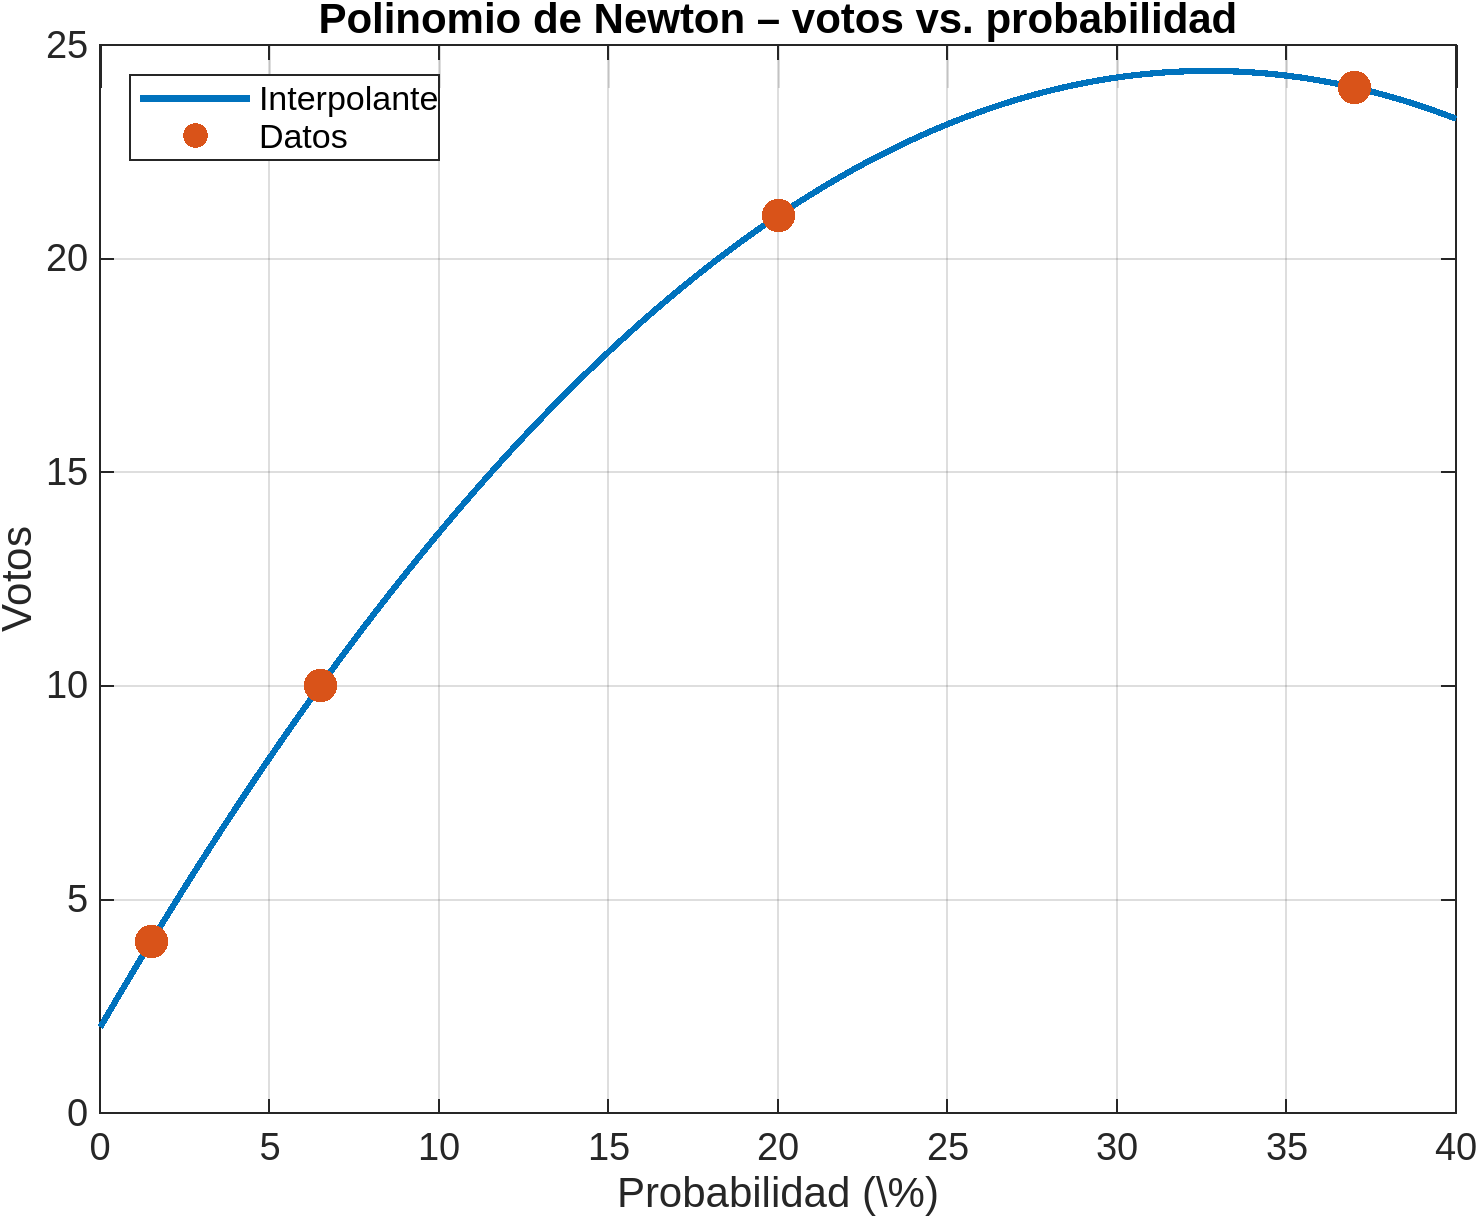
\includegraphics[width=.75\textwidth]{Figures/0. General/PolinomioNewton.png}
    \caption{Polinomio interpolante de Newton (grado 3) y datos de votos
             frente a probabilidad.}
    \label{fig:poly_newton}
\end{figure}

\hfill\break

\section{3. (1 pt) ¿Estafaron a Sentry?}

Sentry está muy puto por su derrota, y afirma que lo estafaron con ese sistema
de ecuaciones, ya que no entiende ¿cómo es posible que el método siempre
converja (aún con cualquier cambio en $cc$)?, sabiendo que el método de SOR es tan
inestable. Explique a Sentry a qué se debe esta convergencia absoluta del
método, según lo visto en clase. Evite que se empute más y termine
desapareciendo a todo el mundo.\\

\hfill\break

No, Sentry, desafortunadamente no hubo trampa.  
El método SOR siempre llega al mismo resultado en este problema porque la
matriz \(A\) de los votos tiene un rasgo muy favorable:

\[
\text{cada número de la diagonal es, en valor absoluto, mayor que la suma de
los demás números de su fila.}
\]

Cuando eso pasa se dice que la matriz es **“dominante en la diagonal”** y los
métodos iterativos (Jacobi, Gauss-Seidel y, por supuesto, SOR) \emph{siempre}
convergen, uses el valor que uses para \(cc\) y empieces donde empieces.

En palabras simples:
\begin{itemize}
\item Los números grandes de la diagonal "mandan" y obligan al
  algoritmo a estabilizarse.  
\item Cambiar un \(10\) por un \(9\) o un \(11\) en las posiciones
  \(\pm cc\) no supera a la diagonal, así que la dominancia se mantiene.  
\item Con un factor de relajación \(0<w<2\) —el nuestro es \(1.15\)— SOR
  está garantizado a acercarse cada vez más a la solución real.
\end{itemize}

Sin importar el arranque ni el valor exacto de \(cc\),
los errores iban disminuyendo hasta quedar por debajo de la tolerancia.
En resumen, la convergencia “absoluta” se debe a la forma tan
bien balanceada (dominante) de la matriz, no a ningún truco vaticano.
